\chapter{Data}
\label{ch:data}

\marginpar{Perché non devo dire che non ho preso nuovi dati? Mi sembra una
cosa da specificare.}

We drew on two types of datasets: 1)~ data collected with the Proto0 DarkSide
prototype at CERN, and 2)~data collected with a cryogenic test stand at
Laboratori Nazionali del Gran Sasso (LNGS).

\marginpar{Cosa sono le biscioline?}

Both datasets contain digital traces of photodetector modules (PDMs) output,
divided in continuous chunks of fixed length that we call ``events''.
Optionally, a pulsed laser is shone at the detector and the temporal window of
the event waveform is synchronized with the laser.

\section{Proto0}
\label{sec:dataproto0}

Proto0 is a small prototype of time projection chamber (TPC) in liquid argon
(LAr). It was built and operated in CERN building 182 in 2019, and now will be
moved and operated again in Napoli in 2021. Information is provided in the CERN
wiki page \cite{proto0}. Note that the descriptions in
\cite[sec.~4.3.2]{luzzi2020} and in the Yellow Book \cite[65]{aalseth2018}
contain outdated information relative to the status of the setup when the data
we are considering was recorded.

\marginpar{La correzione dice di cancellare la reference, e poi di aggiungerla,
quindi non ho capito.}

The TPC size is $\SI{30}{cm} \times \SI{30}{cm} \times \SI{20}{cm}$. On top of
the TPC sits a photodetector unit (PDU), i.e., data transmission electronics
plus a motherboard. This specific one is dubbed ``Motherboard 2'' (MB2), and
consists of a matrix of $5\times 5$ PDMs. The silicon photomultipliers (SiPMs)
Tiles mounted in the PDMs were fabricated by Fondazione Bruno Kessler (FBK) in
2019. The tiling scheme of the motherboard is shown in \autoref{fig:pdmadcch},
while in \autoref{fig:proto0} there are some photos of the apparatus.

\marginpar{A Stracka: il downsampling l'hai fatto tu, giusto? Che downsampling
è, decimazione, media, o più complicato?}

The PDM outputs are each sent to a channel of a CAEN V1725 analog to digital
converter (ADC) board. The ADC has \SI{16}{bit} and sampling frequency
\SI{250}{MSa/s}, downsampled in software to \SI{125}{MSa/s} to match the
specifics which will be adopted in DarkSide20k. The response of the SiPMs will
be described briefly in \autoref{ch:snr} and more in detail in
\autoref{ch:anal}.

Of the Proto0 data, we used only a run collected with the PDMs biased below
breakdown voltage and thus almost insensitive to light. So the waveforms
contain only electrical noise. We analyzed 1000~events, each \SI{0.5}{ms} long.
In \autoref{tab:proto0meta} we list for reference the conditions for this run.
A persistence plot of the data for Tile~53 is shown in
\autoref{fig:hist2dtile53}.

\begin{figure}
    
    \widecenter{
        \newlength\protoheight
        \setlength\protoheight{7.5cm}
        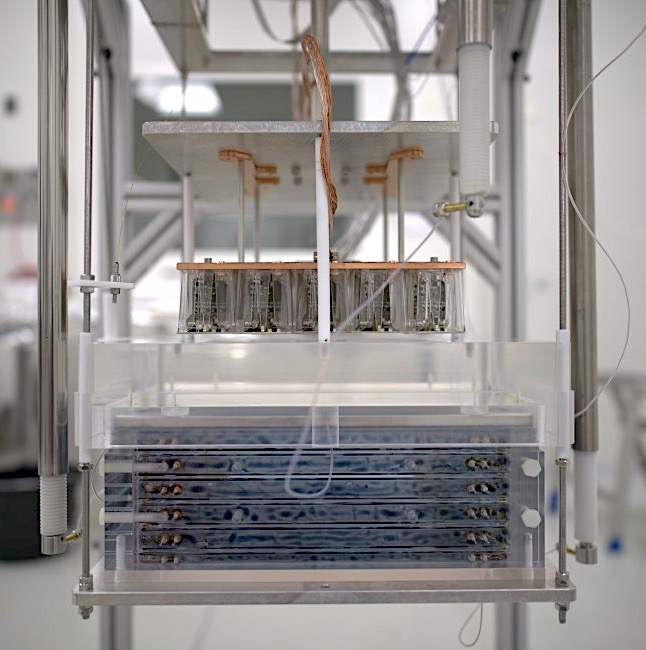
\includegraphics[height=\protoheight]{proto0-1}
        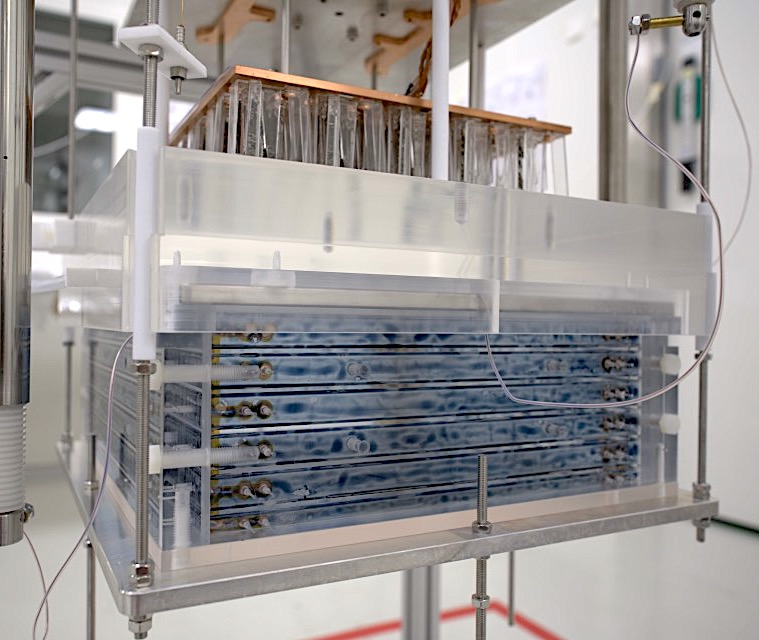
\includegraphics[height=\protoheight]{proto0-2}
    }
    
    \caption{\label{fig:proto0} The Proto0 TPC outside of the cryostat. Photos
    by Tom Thorpe (GSSI) \cite{proto0photos}. When in the cryostat, the whole
    object is completely submerged in LAr. Inside the bluish box there is a
    uniform electric field pointing top to bottom. The stripes on the sides are
    conductive and are the steps of a voltage divider, to create boundary
    conditions that keep the field uniform even near the borders. The metal
    frame visible just over the blue box, behind the semitransparent plastic,
    is the support of the grid used to create an high field region above it up
    to the anode. That region is contained in a ``gas pocket'', i.e., something
    like a cup kept upside-down underwater. The pocket is kept filled with
    gaseous argon. The copper frame on the top supports the PDMs, with their
    characteristic plastic case holding the front end board (FEB) attached
    orthogonally to the SiPMs Tile.}
    
\end{figure}

\begin{figure}
    
    \widecenter{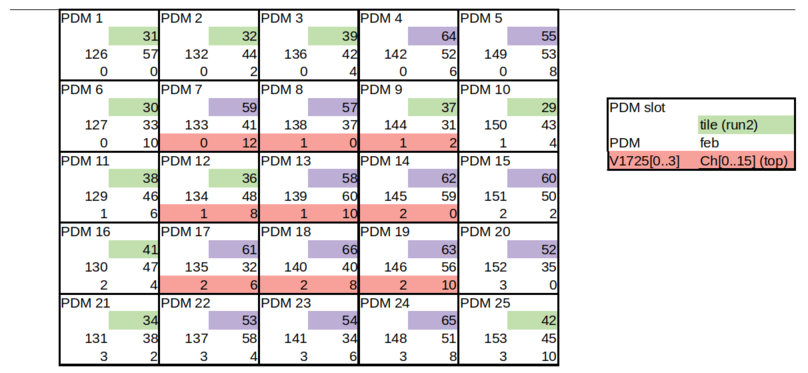
\includegraphics[width=1.2\textwidth]{PDMadcCh}}
    
    \caption{\label{fig:pdmadcch} Schematic of the motherboard installed in
    Proto0, showing the SiPM Tile identification number of each PDM and the ADC
    channels. The color of the Tile number sets apart the two set of SiPMs
    used: green ``run2'' have a higher breakdown voltage than violet ``run4'';
    being all operated at the same bias, the run2 Tiles have overvoltage
    \SI{5.5}{V} while run4 \SI{6.5}{V}. The PDMs marked in red are the inputs
    of the data trigger, which is not used in the data we consider.}

\end{figure}

% info on Proto0:
% Report_v1 Report on DAQ operation of MB1 test setup at CERN.pdf, page 1 and 2
% Kish_DS_CollabMeeting-Nov2019_Naples_Proto0 DarkSide Proto-0 activities.pdf
% Darkside_general_meeting_Napoli_Last updates on the tests and the next steps toward DS Proto 1ton.pdf, pages 12--18

\clearpage
\section{LNGS}
\label{sec:lngsdata}

\marginpar{``test stand'' è inglese o è il software della NI (labview)?}

We also used laser-run data collected at LNGS with a test stand built to
characterize individual SiPMs or Tiles, briefly described in the Yellow Book
\cite[34]{aalseth2018}, and presented in greater detail in \cite{acerbi2017}
and \cite[ch.~3]{savarese2018}. It achieves a temperature stability of
\SI{0.1}K and accuracy \SI{3}{K} in the operative range \SI{40}{K} to
\SI{300}{K}. The digitizer is a CAEN V1751.

\marginpar{Perché non devo dire che non sappiamo davvero tutte le specifiche?}

\marginpar{Devo dire che la luce laser viene diffusa.}

These datasets were collected between 2018 and 2021 by Lucia Consiglio. They
contain all the FBK Tiles used in Proto0 apart from Tile~55 (data from
2018--2019), plus other newer Tiles produced by LFoundry, Tiles~15, 21, 22,
and~23 (data from 2020--2021). The data was retrieved from the bookkeeping
directories \nolinkurl{SiPM/Tiles/FBK/NUV/MB2-LF-3x/} and
\nolinkurl{SiPM/Tiles/LFOUNDRY/pre-production-test/}. The directory name
\nolinkurl{MB2-LF-3x} stands for ``Motherboard 2, low field, triple doping''.
The data for all Tiles are collected using the same reference FEB.

\marginpar{A Stracka: mi hai fatto togliere gli url dei dati, però sul README
del codice ci sono ancora, li devo cancellare?}

The events are laser-triggered and recorded in \texttt{wav} files. Each file
contains the Tile output, and in most runs there is also the recorded laser
trigger in an additional channel, containing a square pulse marking the trigger
location, which occurs at the same place relative to the event start varying in
a \SI{23}{ns} range (see \autoref{fig:triggerhist}). Of the two-channels files
we used, the channel layout is 0:PDM, 1:trigger for FBK, swapped for LFoundry.

\stracka{As part of the preprocessing, we sort the channels in a consistent
manner (o qualcosa del genere)}

The format of the \texttt{wav} files is the following. The files are arrays of
16~bit signed integers, divided into events. Each event starts with 20 values
of metadata, followed by \num{15001} values for each channel. The ADC
resolution is 10~bit, so the values are always in the range 0 to~1023. The
sampling frequency is \SI{1}{GSa/s}.

\marginpar{Perché non devo scrivere il formato dei metadati, visto che mi
sarebbe stato utile saperlo quando ho cominciato la tesi?}

Persistence plots of the data for tiles 15, 21, 53, 57 and~59 are shown in
\autoref{fig:hist2dtile155759}, \ref{fig:hist2dtile21}, \ref{fig:hist2dtile53},
and~\ref{fig:hist2dtile57}.

\marginpar{Ho corretto gli errori ortografici nella tabella di Proto0, ma
non erano miei, stanno nell'excel di Proto0}

\begin{table}
    \widecenter{
        \begin{tabular}{llll}
            \toprule
            Field                 & Value        & Field                        & Value            \\
            \cmidrule(r){1-2}                    \cmidrule(l){3-4}              
            run                   & 886          & gas pocket                   & ON               \\
            date(dd-mm)           & 5-11         & laser intensity              &                  \\
            run type              & baseline run & trigger                      & external (50 Hz) \\
            Quality               & good         & trigtime (\si{\micro s})     & 100              \\
            Problem               &              & post-trigger (\si{\micro s}) & 400              \\
            Nevents (k)           &              & Time gate  (\si{\micro s})   & 500              \\
            Edrift (V/cm)         & 200          & PDM Coincidence              &                  \\
            Eextraction (kV/cm)   & 2.8          & Threshold extent (ns)        & 80               \\
            SiPM bias voltage (V) & 50           & TPC pressure (mbarg)         & >450             \\
            \bottomrule
        \end{tabular}
    }
    
    \caption{\label{tab:proto0meta} Metadata for the Proto0 baseline run~886.}
    
\end{table}
